% chktex-file 21
% \subsection{研究路线}\label{sec:ch3:method}

本章首先通过千年时间尺度上的数据和记录,将气候的周期性变化、日益增长的人类活动压力各自对流域系统的影响相剥离,识别人类活动驱动因素超越气候周期波动影响的时期,作为人水关系稳态转换的稳态转化关键阶段。
水沙关系的变化是历史时期人水关系反馈过程影响最大的关键变量,本章重点关注气候周期性变化和人类活动对流域产水、产沙的影响、以及二者之间的相互影响,通过选定能在反映黄河历史产水量、产沙量的获取的可靠数据,厘定黄河流域水沙关系变化的时期和过程,将水沙关系受人类主导超过受气候周期影响的时间,作为识别黄河流域人水关系变化的关键时期。

\begin{figure}[!htb] % use float package if you want it here
    \centering
    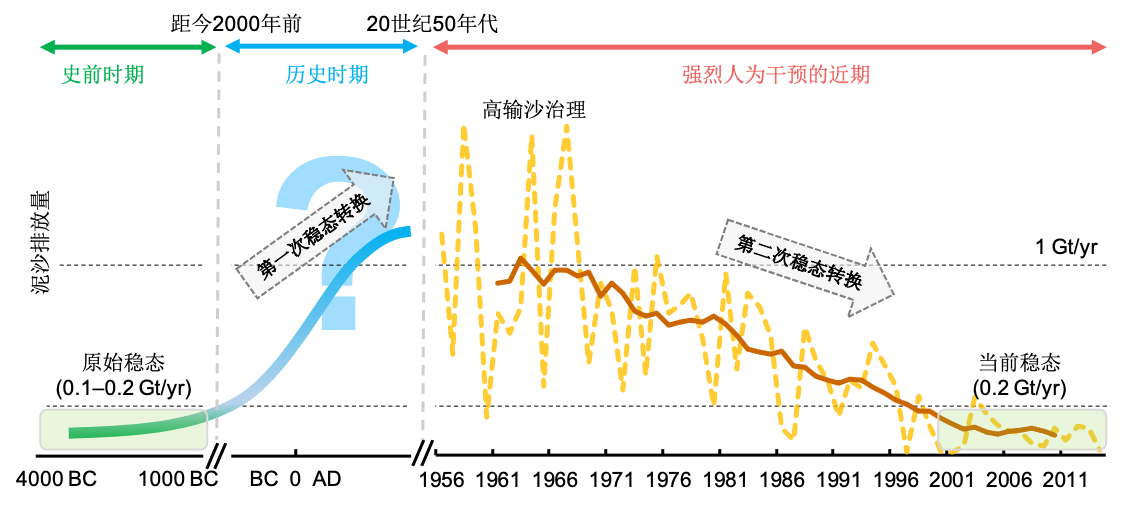
\includegraphics[width=\textwidth]{img/ch3/ch3_why_regime_shift.png}
    \caption{黄河流域历史时期水沙特征变化}\label{fig:ch3:why_regime_shift}
    % 第一次稳态转换发生在历史时期~\textbf{A},从原始状态进入了人类活动主导社会-水文二元循环的流域系统~\textbf{D},但稳态转换的发生过程~\textbf{B}以及历史时期流域系统的人水关系模式\textbf{C}尚不明晰。
\end{figure}

\subsection{稳态转换识别框架}\label{sec:ch3:approach}

% 在历史时期的黄河流域,由于缺乏对流域的系统性认识,不断增长的人为压力带来的影响主要是中游黄土区的开垦进而导致输沙量的提升\cite{wu2020a}。
% 基于上述研究路线,针对此次待识别的稳态转换特点,
本研究设计了如图\ref{fig:ch3:regime_shift_detect}所示的稳态转换识别框架。
周期性气候变化和不断增长的人为因素(主要是中游易侵蚀区的粮食生产)共同驱动着产沙量、产水量两个关键特征的变化,并进一步在流域内触发一系列影响因素变化。
在气候湿润时期,土壤侵蚀和径流会因更丰富的降水而增加,通常导致产水量和产沙量同时上升,因此二者也存在一定的正相关\cite{GeQuanSheng2011}。
随着人类活动压力增大,开垦通常造成粮食产量增加、供养更多人口,但减少植被的覆盖范围,加剧水土流失并导致产沙量增多\cite{wu2020a}。
本章研究首先识别潜在的气候变化/人类活动驱动时期,进而通过分析与产沙过程、产水过程相关联的三类影响因素在驱动期前后的综合变化趋势(图\ref{fig:ch3:impacts_diagram})找到“产沙量增加比产水量增加更显著”的稳态转化时期。

\begin{figure}[htb] % use float package if you want it here
    \centering
    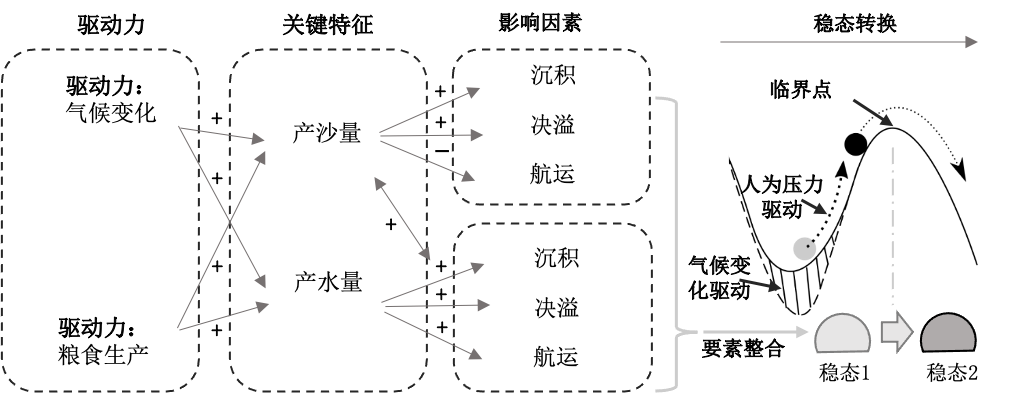
\includegraphics{ch3/ch3_workflow.png}
    \caption[黄河历史时期水沙特征的稳态转换识别框架]{黄河历史时期稳态转换识别的框架。气候变化和粮食生产是致使稳态转换发生的潜在驱动力;稳态转换发生时影响的关键是产沙量和产水量;二者的变化又会触发流域一系列影响因素变化。灰色箭头及其旁边的符号表示消极或者积极的影响路径;在驱动力推动系统接近临界点时,所有受影响因素经整合后会展示稳态转换是否发生。}\label{fig:ch3:regime_shift_detect}
\end{figure}

% \subsection{驱动时期识别方法}

本章研究首先识别不同驱动力(潮湿气候/人类活动)所主导的时段,然后分析该时段之前、之中、之后受到影响的指标如何变化。
由于干燥和潮湿的气候在中国往往以约100年为周期\cite{GeQuanSheng2011},因此本章研究以100年最低阈值来检测气候驱动时段(Climate-driven Periods, CDPs)。
本章研究选取了反映潮湿环境和极端降水的湿度数据和洪水频率数据,作为识别过去两千年中历史气候驱动时段出现的指标。
在每个100年时段中,如果洪水的频次高于干旱事件频次,并且累积湿度距平在上升,则可以认为是典型的气候驱动时段。

人类活动带来的主要压力来自于黄河中游的人口增长以及农业扩张。
尽管目前没有精确的人口数据,但中国历史人口变化的趋势已在一些基于户籍统计的历史重建资料中得到反映(详见表\ref{tab:data_source})。
此外,农牧交错带北界的移动也是人类活动的重要特征。本章研究将其作为人类活动驱动时段(Human-driven Periods, HDPs)的辅助识别指标。
由于人口的增长不一定直接伴随着农业开垦面积的扩张,仅当农业人口增长和农牧交错带北界的移动同时发生时,才能认为是人类活动驱动时段。

\subsection{数据来源}

% 本章研究的主要挑战是数据可得性。因此,研究方法和指标必须根据可靠的数据进行设计。
本研究通过梳理前人在沉积学、气候学、历史学等领域的成果,获取了公开发表、质量可靠的数据,并对其进行了处理和再分析。
% 根据本章研究中的用途,数据集可分为两大类:驱动力数据(依据其与“水沙变化”的关系,又可以分为“气候驱动力”、“人类活动驱动力”、“混合驱动力”三大类)、受黄河水沙特征变化影响的数据。
数据集的可靠程度因数据来源和数据丰富程度的不同而有所差异(表\ref{tab:data_source})。
(1)干旱和洪涝频率:记录了中原、华北平原地区的干旱、洪涝灾害的频次,每五十年为一个时期,来源为官方和地方的史料记录,数据的可信度根据不同历史时段的材料丰富程度有所差异。
(2)湿润指数累计距平:根据史料中与湿度相关的记录,评估历史时期气候湿润程度的等级,来源为官方和地方的史料记录,数据的可信度根据不同历史时段的材料丰富程度有所差异。
(3)黄河中游人口数量:利用史料记录推断的黄河中游人口,来源为历史户籍注册信息,数字不精确但可以反映趋势以供纵向比较。
(4)农牧交错带的北界位置:记录了农牧交界线距离潼关所在维度的平均距离,来源为中国历史地图集,时间采样点比较少,但每个点的位置数据较为可信。
(5)三门峡峡谷航运数据:记录了三门峡航运通行难易程度的等级,来源为官方和地方的史料记录,数据从可靠的史料来源获得,但存在数据缺失情况。
(6)黄河下游决溢数据:记录了黄河下游堤防崩溃的次数,来源为官方和地方的史料记录,数据的可信度根据不同历史时段的材料丰富程度有所差异。
(7)黄河古河道沉积速率:结合历史地图和取样测定的黄河古河道沉积速率,来源为沉积样本,样本所在的古河道时间跨度越长样本越精确。

% Table generated by Excel2LaTeX from sheet 'Sheet1'
\begin{table}[hbt]
  % \centering
  % \begin{minipage}[t]{0.8\linewidth}
  \caption[千年尺度黄河稳态转换识别的数据来源]{千年尺度黄河稳态转换识别的数据来源。}
    % \begin{tabular}{llllll}
    \begin{tabularx}{\textwidth}{ p{2cm} L p{5cm} L p{3cm} L}
    \toprule
    数据集   & 类型    & 描述    & 原始材料  & 可信度   & 参考 \\
    \midrule
    干旱和洪涝频率 & 气候驱动力 & 每五十年为一个时期,分别统计中原、华北平原地区的干旱、洪涝灾害的频次 & 官方和地方的史料记录 & 根据历史材料的丰富程度,在不同时期的可信度是不一致的 & 葛全胜,2011 \cite{GeQuanSheng2011} \\
    湿润指数累计距平 & 气候驱动力 & 根据史料中与湿度相关的记录,评估历史时期气候湿润程度的等级 & 官方和地方的史料记录 & 根据历史材料的丰富程度,在不同时期的可信度是不一致的 & Zheng,2006 \cite{zheng2006} \\
    黄河中游人口数量 & 人类活动驱动力 & 利用史料记录推断的黄河中游人口 & 历史户籍注册信息 & 数字不精确但可以反映趋势以供纵向比较 & Chen et al., 2012 \cite{chen2012} \\
    农牧交错带的北界位置 & 混合驱动力 & 农牧交界线距离潼关所在维度的平均距离 & 中国历史地图集 & 时间采样点比较少,但每个点的位置数据较为可信 & 谭其骧,1996 \cite{TanQiXiang1996} \\
    三门峡峡谷航运数据 & 影响$^*$    & 三门峡航运通行难易程度的等级 & 官方和地方的史料记录 & 数据从可靠的史料来源获得,但存在数据缺失情况 & 王守春,1993 \cite{WangShouChun1993} \\ %TODO 这里还需要参考,查证王老师那的书
    黄河下游决溢数据 & 影响    & 黄河下游堤防崩溃的次数 & 官方和地方的史料记录 & 根据历史材料的丰富程度,在不同时期的可信度是不一致的 & Chen et al., 2012 \cite{chen2012} \\
    黄河古河道沉积速率 & 影响    & 结合历史地图和取样测定的黄河古河道沉积速率 & 沉积样本  & 样本所在的古河道时间跨度越长样本越精确 & Xu 2003 \cite{xu2003a} \\
    \bottomrule
    % \end{tabular}%
  \end{tabularx}\\[2pt]
  % \leftalighn
  \footnotesize 注:*影响:指黄河关键特征变化带来的影响。\\\label{tab:data_source}%
  % \end{minipage}
\end{table}%


\subsection{数据处理}

分析稳态转换驱动的数据集时空尺度均已匹配本章研究需要,均不做进一步处理。
反映黄河特征变化带来的影响的三个数据集(黄河古河道沉积速率、洪泛决溢次数、三门峡航运情况)需要按表\ref{tab:ch3_impacts_magnitude}进行半定量化。
由于历史资料难以避免具有不确定性,需要根据上述三个数据集的特点评估它们的置信度并进行整合。本章研究首先按照公式\ref{eq:ch3_credibility}对沉积、决溢和航运三个数据集各自的置信度进行估计:
(1)对于沉积数据,每个数据都是对遗留河床样本沉积速率的平均估计,遗留时间越长的古河床样本的估计值越可靠;
(2)对于决溢数据,它的置信度取决于官方史料的可靠程度,该时期的历史记录更可靠、存留的历史记录更多,则该时期的估计值也更可靠;
(3)由于航运数据出处未给出各时段的史料置信度,所以该数据的置信情况使用时段内航运相关记录的数量进行评估。
最后,将每个数据集的置信度按照极大-极小归一化(公式\ref{eq:ch3_normalize})进行标准化,然后同样划分为三个置信等级。

\begin{figure}[htb] % use float package if you want it here
    \centering
    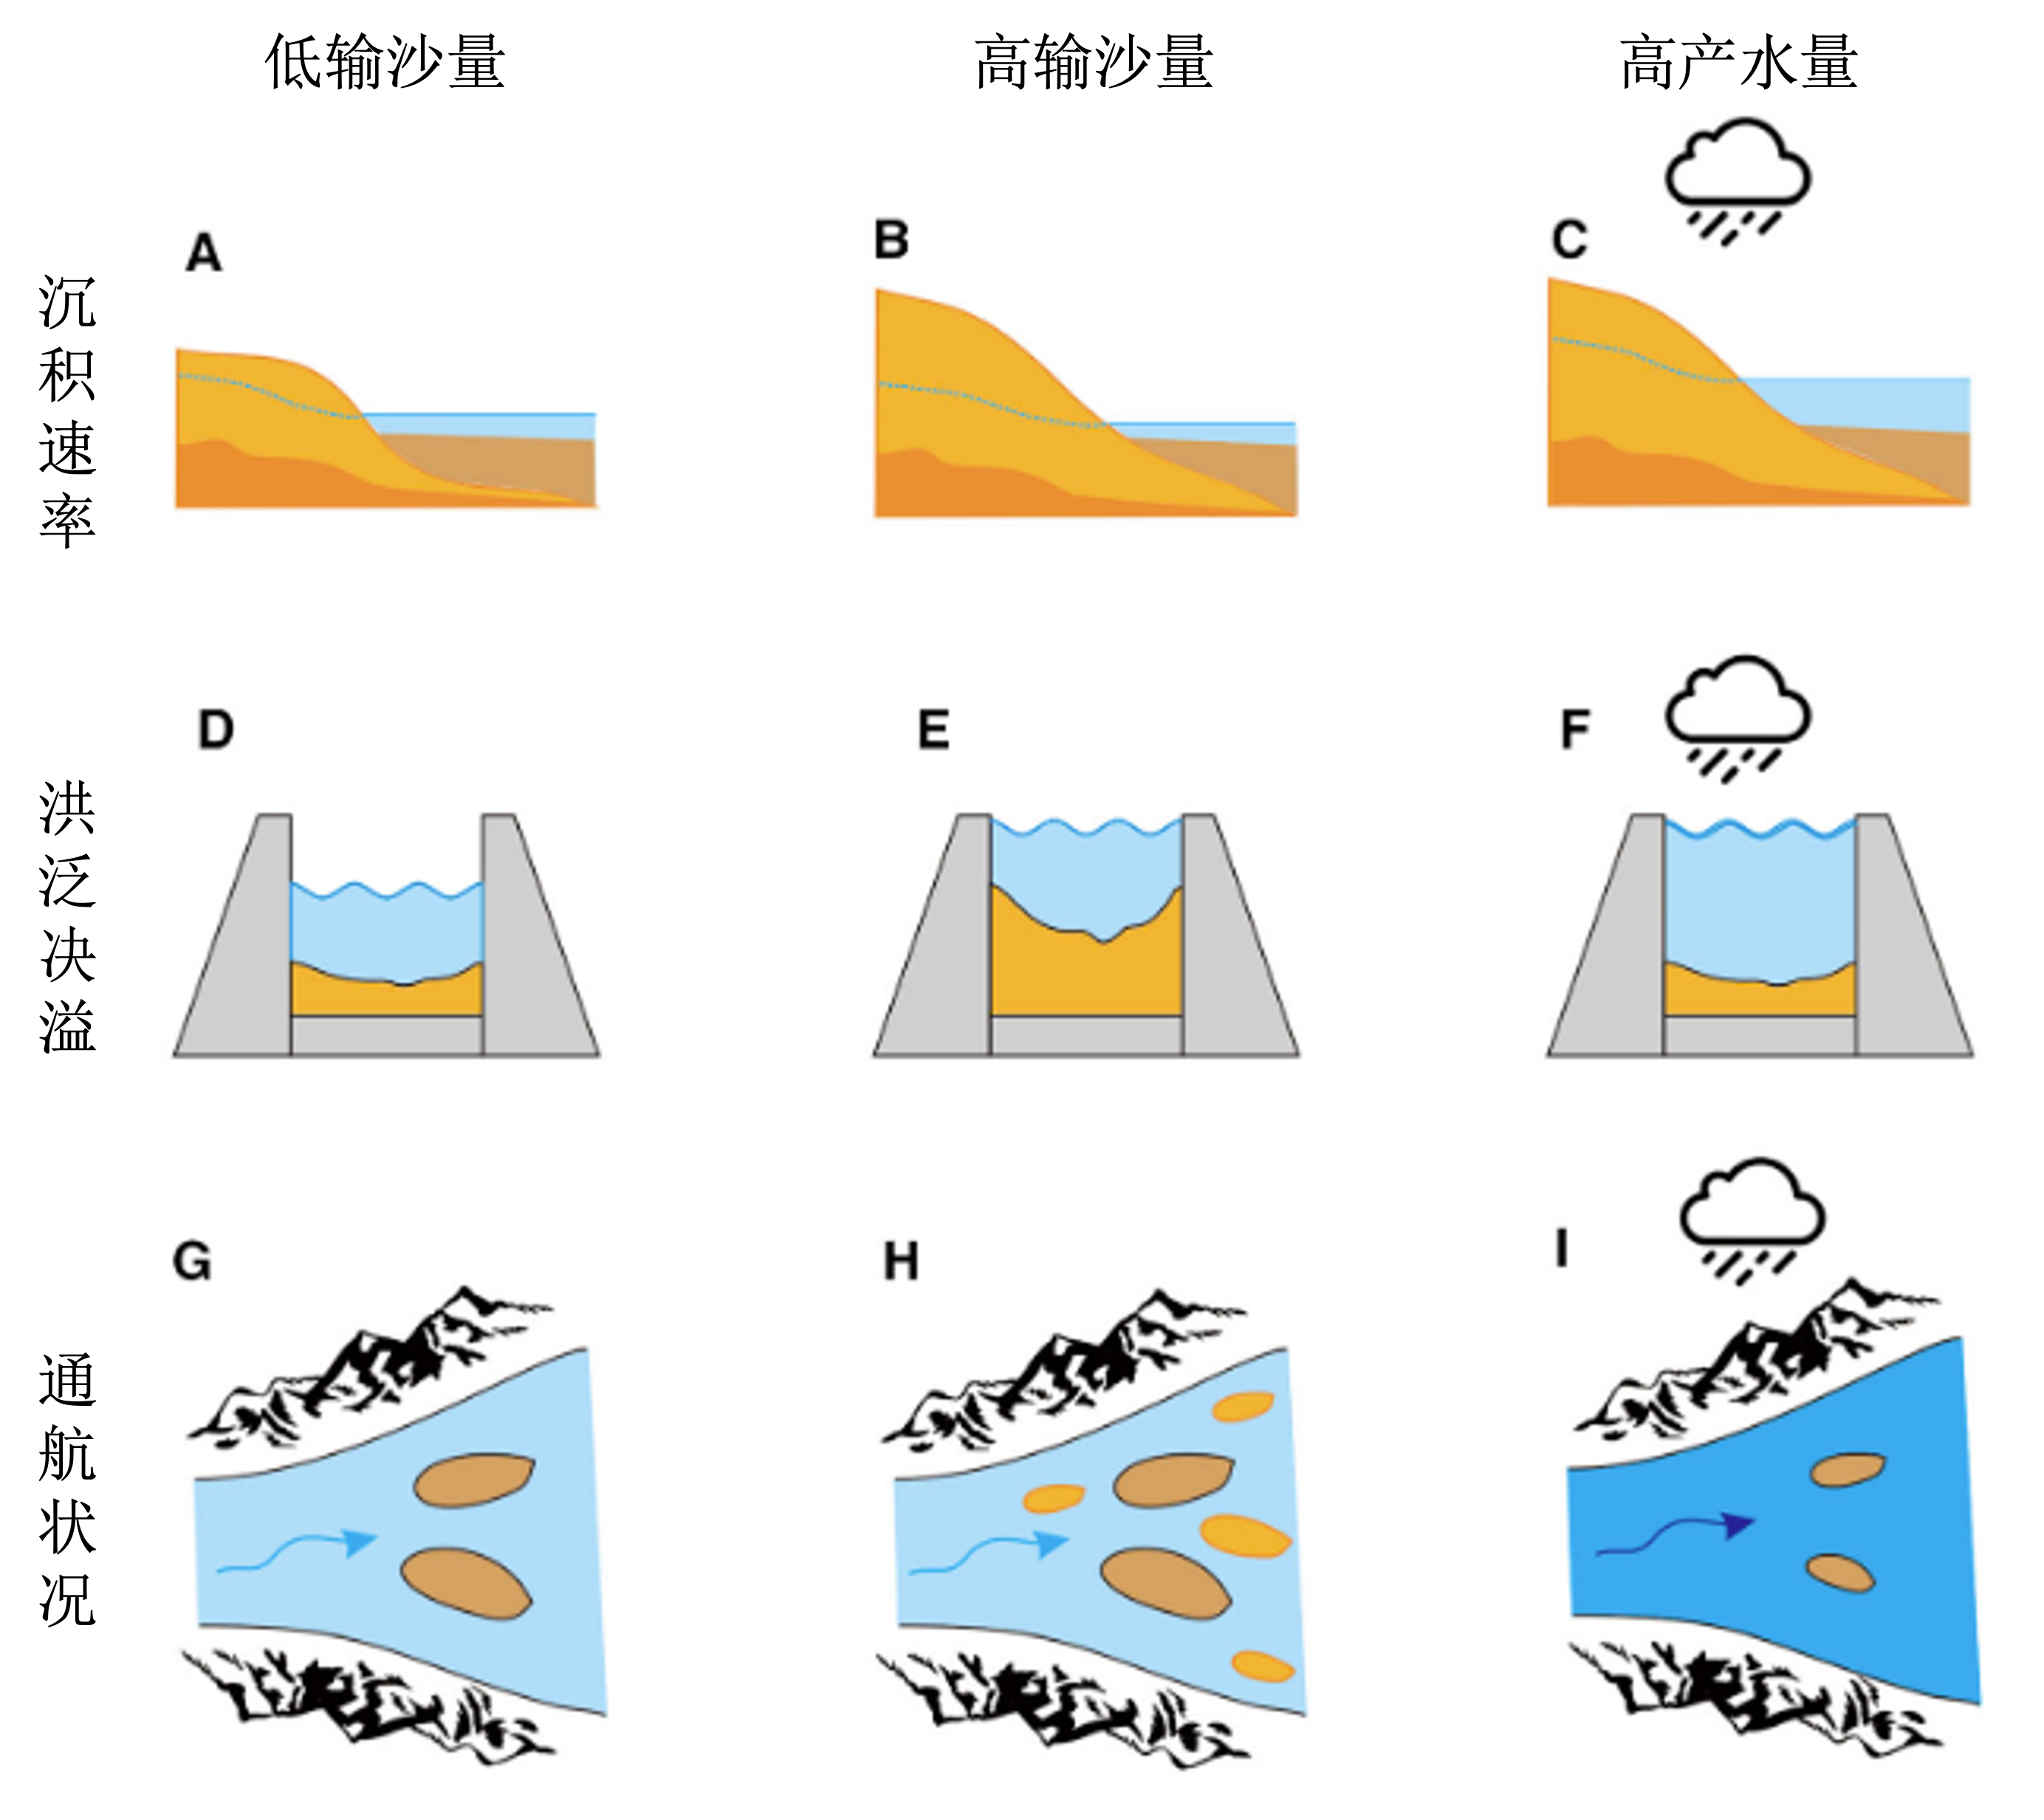
\includegraphics[width=\textwidth]{img/ch3/ch3_impacts_diagram.png}
    \caption[黄河历史产水量和产沙量变化的影响]{黄河历史产水量和产沙量带来的影响。输沙和产水两个主要特征分别对沉积(A-C);决溢(D-F);航运(G-H)的影响。
    (1)沉积数据,产沙量高(从A到B)可能导致下游沉积速率增加\cite{xu2003a};
    (2)洪泛数据,产沙量高(从D到E)或者气候湿润期(从D到F)都有可能导致更多的决溢洪泛\cite{chen2012};
    (3)航运数据,产沙量高(从G到H)会增加浅滩数量,从而使航运变得更加困难,而潮湿的气候时期由于平均径流量变大,三门峡的通航将更加容易\cite{WangShouChun1993}。}\label{fig:ch3:impacts_diagram}
\end{figure}

% Table generated by Excel2LaTeX from sheet '影响强度半定量化'
\begin{table}[!htbp]
    \caption{黄河关键特征变化影响强度的半定量分级}
      \begin{tabularx}{\textwidth}{p{1.5cm} LLL}
      \toprule
      \multicolumn{1}{l}{强度等级} & 古河道沉积速率 & 洪泛决溢频次 & 三门峡航运情况 \\
      \midrule
      1     & $0 \sim 2$ cm/yr & < 10次 / 20yrs & 自由通行 \\
      2     & $2 \sim 4$ cm/yr & 10~20次 / 20yrs & 需要人力辅助 \\
      3     & $\> 4cm/yr$ & >20次 / 20yrs & 完全无法通行 \\
      \bottomrule
      \end{tabularx}%
    \label{tab:ch3_impacts_magnitude}%
\end{table}%


\begin{equation}
    \label{eq:ch3_credibility}
    Credibility_X = 
    \left\{\begin{array}{l}
        \text{[沉积], } 1 / \frac{1}{n} \sum_{i=1}^n T_i\\
        \text{[决溢], } \prod_{i=1}^n C_i\\
        \text{[航运], } N_i
    \end{array}\right.
\end{equation}    

其中$n$均为给定时段内各数据集样本/记录的数量。$T_i$为每个沉积样本所在古河道的时间跨度;$C_i$是每个历史记录所在时段的置信程度(由数据作者给出的评估,详见表\ref{tab:data_source});$N_i$是每个时期航运相关历史记录的数量。

\begin{equation}
    \label{eq:ch3_normalize}
    C_{X, nom}=\frac{C_X-C_{X, \min}}{C_{X, \max}-C_{X, \min}}
\end{equation}

公式\ref{eq:ch3_normalize}中$C_{X}$为参照公式\ref{eq:ch3_credibility}对数据集$X$进行评估后的置信程度,$C_{\min, X}$, $C_{\max, X}$分别为数据的最小值和最大值。$C_{nom}$为归一化后的置信程度。
